% !TeX spellcheck = en_US
\documentclass[letterpaper,12pt,twoside]{report}
\usepackage{fancyhdr}
\usepackage{fullpage}
\usepackage{tikz}
\usepackage{amsmath}

\begin{document}
	\pagestyle{fancy}
	\fancyhf{}
	\fancyhead[L]{Day 20}
	\fancyhead[R]{\textit{The Calendar Project}}
	\fancyfoot[L]{Citations Involved: none}
	
	% Problem
	\paragraph{Problem}
	\begin{quote}
		\textsf{Three vertices of a square in the $xy$-plane have coordinates $(25,26)$, $(15, 2)$,
			and $(8,19)$. What are the coordinates of
			the center of the square?}
	\end{quote}
	
	% Graphics
	\begin{center}
		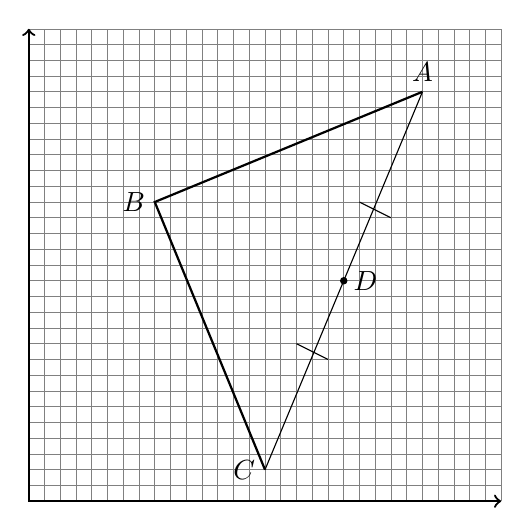
\begin{tikzpicture}[scale=0.2]
		\draw[help lines] (0,0) grid (30,30);
		\draw[<->, thick] (0,30) -- (0,0) -- (30,0);
		
		\draw[thick] (25,26) -- (8,19) -- (15,2);
		\draw (15,2) -- (25,26);
		
		\node[above] at (25,26) {$A$};
		\node[left] at (8,19) {$B$};
		\node[left] at (15,2) {$C$};
		
		\draw[fill=black] (20,14) circle [radius=0.2];
		\node[right] at (20,14) {$D$};
		
		%\draw[fill=black] (32,9) circle [radius=0.2];
		%\node[right] at (32,9) {$E$};
		
		\draw (17,10) -- (19,9);
		\draw (21,19) -- (23,18);
		
		%\draw[dashed] (8,19) -- (32,9);
		%\draw[dashed] (15,2) -- (32,9) -- (25,26);
		%\draw (15,15) -- (16,17);
		%\draw (24,11) -- (25,13);
		\end{tikzpicture}
	\end{center}
	
	% Reasoning
	\paragraph{Reasoning}
	\begin{quotation}
		
		A square is a rectangle, rhombus, and a parallelogram (3). A parallelogram's diagonals bisect each other (1); given the endpoints of diagonal $\overline{AC}$ (shown above), its midpoint $D$ is where the other diagonal would bisect it. Since a rectangle's diagonals are congruent (2), their midpoint $D$ is equidistant to the square's vertices. Since a square is both equiangular and equilateral by definition, it is a regular polygon. Since the center of a regular polygon is equidistant from the vertices by definition (4), $D$ is the center of the square. Its coordinates are determined as follows:
		
		\begin{center}
			\begin{tabular}{l | l}
				$(\frac{15+25}{2},\frac{2+26}{2})$ & Apply the Midpoint Formula \\
				$(\frac{40}{2},\frac{28}{2})$ & Evaluate the numerators \\
				$(20,14)$ & Simplify
			\end{tabular}
		\end{center}
	
		The solution to this problem is $\boxed{(20,14)}$.
	\end{quotation}
	
	\paragraph{External References}
	
	\begin{enumerate}
		\item Textbook Ch. 6, Pg. 392: Properties of Parallelograms
		\item Textbook Ch. 6, Pg. 408: Properties of Rectangles
		\item Textbook Ch. 6, Pg. 410: Verifying Properties of Squares
		\item Textbook Ch. 9, Pg. 601: Definition of the center of a regular polygon
	\end{enumerate}
	
\end{document}